\documentclass[11pt,a4paper,reqno, dvipsnames]{article}
\usepackage[utf8]{inputenc}
\usepackage[T1]{fontenc}
\usepackage{mathtools, amsmath, amsthm, amsfonts, amssymb}
\usepackage{tikz}
\usetikzlibrary{arrows.meta}
\usetikzlibrary{positioning, shapes.multipart, arrows}
\usetikzlibrary{shapes, fit}
\usepackage{pgfplots}
\pgfplotsset{compat=1.18}

\begin{document}

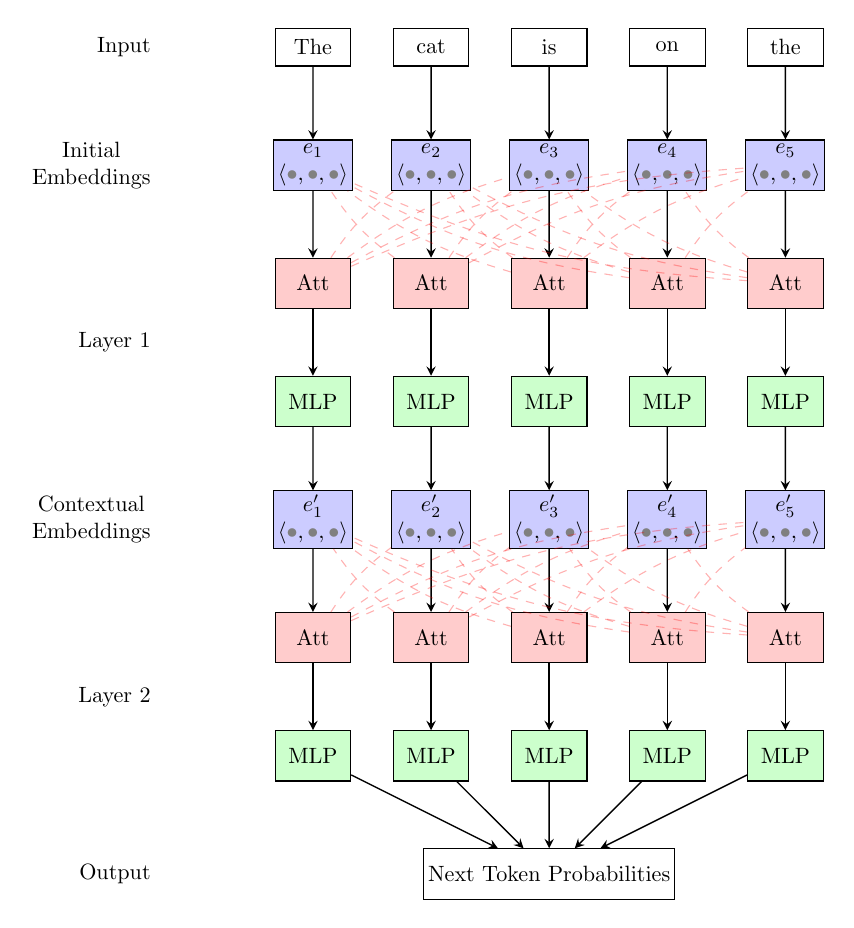
\begin{tikzpicture}[
  every node/.style={font=\rmfamily, align=center, inner sep=0.2em, scale=0.8},
  token/.style={rectangle, draw, minimum width=1.2cm, minimum height=0.6cm},
  embedding/.style={rectangle, draw, fill=blue!20, minimum width=1.2cm, minimum height=0.8cm},
  attention/.style={rectangle, draw, fill=red!20, minimum width=1.2cm, minimum height=0.8cm},
  MLP/.style={rectangle, draw, fill=green!20, minimum width=1.2cm, minimum height=0.8cm},
  output/.style={rectangle, draw, minimum width=3cm, minimum height=0.8cm},
  arrow/.style={->, >=stealth, line width=0.5pt}
]
% Input tokens
\foreach \word [count=\i] in {The, cat, is, on, the} {
  \node[token] (input-\i) at (\i*1.5, 0) {\word};
}
% Initial Embeddings
\foreach \i in {1,...,5} {
  \node[embedding] (emb-\i) at (\i*1.5, -1.5) {$e_\i$ \\ {$\langle \textcolor{gray}{\tiny\bullet}, \textcolor{gray}{\tiny\bullet}, \textcolor{gray}{\tiny\bullet} \rangle$}};
  \draw[arrow] (input-\i) -- (emb-\i);
}
% First Layer
\foreach \i in {1,...,5} {
  \node[attention] (att1-\i) at (\i*1.5, -3) {Att};
  \node[MLP] (MLP1-\i) at (\i*1.5, -4.5) {MLP};
  \draw[arrow] (emb-\i) -- (att1-\i);
  \draw[arrow] (att1-\i) -- (MLP1-\i);
}
% Attention connections in first layer
\foreach \i in {1,...,5} {
  \foreach \j in {1,...,5} {
    \ifnum\i=\j\else
      \draw[red, dashed, opacity=0.3] (att1-\i) to[bend left=10] (emb-\j);
    \fi
  }
}
% Second round of embeddings after Layer 1
\foreach \i in {1,...,5} {
  \node[embedding] (emb2-\i) at (\i*1.5, -6) {$e'_\i$ \\ {$\langle \textcolor{gray}{\tiny\bullet}, \textcolor{gray}{\tiny\bullet}, \textcolor{gray}{\tiny\bullet} \rangle$}};
  \draw[arrow] (MLP1-\i) -- (emb2-\i);
}
% Second Layer
\foreach \i in {1,...,5} {
  \node[attention] (att2-\i) at (\i*1.5, -7.5) {Att};
  \node[MLP] (MLP2-\i) at (\i*1.5, -9) {MLP};
  \draw[arrow] (emb2-\i) -- (att2-\i);
  \draw[arrow] (att2-\i) -- (MLP2-\i);
}
% Attention connections in second layer
\foreach \i in {1,...,5} {
  \foreach \j in {1,...,5} {
    \ifnum\i=\j\else
      \draw[red, dashed, opacity=0.3] (att2-\i) to[bend left=10] (emb2-\j);
    \fi
  }
}
% Output probabilities
\node[output] (output) at (4.5, -10.5) {Next Token Probabilities};
\foreach \i in {1,...,5} {
  \draw[arrow] (MLP2-\i) -- (output);
}
% Labels
\node[left] at (-0.5, 0) {Input};
\node[left] at (-0.5, -1.5) {Initial\\Embeddings};
\node[left] at (-0.5, -3.75) {Layer 1};
\node[left] at (-0.5, -6) {Contextual\\Embeddings};
\node[left] at (-0.5, -8.25) {Layer 2};
\node[left] at (-0.5, -10.5) {Output};
\end{tikzpicture}

\end{document}